\section{Study Settings}

%\kn{This paragraph requires a motivation. The details of Boa's study must be described upfront. Something like "Boa et al.'s study performs ..... Since their study also involved a static analysis component whose impact was not measured, we perform a non-exact replication to understand the impact static analysis may have had in the results...}

\kn{Here it is extremely obvious and clear that we explore a very specific kind of interaction between static and dynamic analysis. a.k.a effect of taint analysis on sandboxes. But in the introduction we kind of use the general S-D interaction and this problem interchangeably. I have left a comment at the introduction.}
Our research work aims to better understand
the use of static analysis to mine Android sandboxes
and explore the benefits of combining taint analysis
with the mine sandbox approach for identifying malicious
behavior. 
On the one hand, Jamrozik et al. suggest that a 
static analysis approach for mining sandboxes
might be ineffective---due to \emph{overapproximation
problem}~\cite{DBLP:conf/icse/JamrozikSZ16}.
However, to the best of our knowledge,
there is no empirical study comparing
static and dynamic analysis for mining sandboxes.
On the other hand, the \blls explored the mining sandbox approach by comparing
the performance of five {\bf dynamic analysis tools} (DroidMate, DroidBot, PUMA,
GUIRipper, and Monkey) for identifying
malicious behavior. Nonetheless, their
research also involved an external static analysis component (DroidFax)
whose impact on the results was not measured---in terms of malware
identification. 
This lack of understanding about the implications of
static analysis for mining sandboxes motivates
our research, which investigates the following research questions.

\begin{enumerate}[(RQ1)]

\item What is the impact of the DroidFax static analysis algorithms on the results of the \blls?
  We estimate the impact in terms of the number of detected malwares. 
  
  
 \item What is the effective performance of each sandbox, in terms of the number of detected malware, when we
   discard the contributions of the DroidFax static analysis algorithms?

 \item What are the benefits of using taint
   analysis algorithms to complement the dynamic analysis approach for mining sandboxes,
   in terms of additional malwares identified?
\end{enumerate}

%\kn{Droidfax comes out of nowhere. We should introduce this or if already introduced earlier, remind the readers of where it stands with the Bao study in the first line of this section when describing boas study}

Answering the research questions RQ1 and RQ2 allows us to better
understand the relevance of combining static
and dynamic analysis for mining Android sandboxes. Moreover,
exploring RQ1 and RQ2 can reveal 
a possible overestimation of the performance of the
dynamic analysis tools in the \blls. Answering research question RQ3
allows us to open up the possibility of finding new strategies for malware detection, complementing the performance of
dynamic analysis through the use of static analysis algorithms.
We conducted two empirical studies to answer the research questions above. We address
the research questions RQ1 and RQ2 in the
first empirical study, whose goal is to conduct a non-exact replication of
the \blls. We conduct the first empirical study using
DroidXP~\cite{DBLP:conf/scam/CostaMCMVBC20} (Section~\ref{sec:droidxp}), a
tool that simplifies the execution of experiments
that compare the performance of dynamic analysis tools
in the task of identifying malwares, using a mining sandbox
approach. We present the study settings of the first
empirical study in Section~\ref{sec:set1}.
In the second empirical study we use
FlowDroid~\cite{DBLP:conf/pldi/ArztRFBBKTOM14} to investigate the 
suitability of taint analysis algorithms to complement the mining sandbox
approach for identifying malwares, and thus it targets our third
research question (RQ3). We present the settings of the second
empirical study in Section~\ref{sec:set2}. 


\subsection{The DroidXP benchmark}\label{sec:droidxp}

We designed and implemented DroidXP to systematically assess and compare the
performance of test generation tools for mining android sandboxes. It allows
the integration and comparison of test case generation tools for mining sandboxes, and simplifies
the reproduction of the studies. DroidXP relies on a
simple \emph{Command Line Interface} (CLI) that simplifies the integration
of different test generation tools and favors the setup and execution 
of the experiments. DroidXP also relies on DroidFax, which instruments
Android apps and collects relevant information about
their execution, including the set of sensitive APIs a given
app calls during a test execution. DroidFax also collects
inter-component communication (ICC) using  static
program analysis.

The DroidXP CLI provides commands for listing all test case
generation tools (executing the project with the option ``list-tools'') that had been
integrated into the tool and commands for executing the experiments. An
\emph{experiment run} can be configured according to several parameters, including:

\begin{itemize}
    \item \texttt{-tools}: Specifies the test tools used in the experiment
    \item \texttt{-t}: Specifies the threshold (in seconds) for the execution time in the experiment
    \item \texttt{-r}: Specifies the number of repetitions used in the experiment
    \item \texttt{-output-format}: Specifies the output format
    \item \texttt{--debug}: Specifies to run in DEBUG mode (default: false)
    \item \texttt{--disable-static-analysis}: Disable DroidFax static analysis phase (default: false)
\end{itemize}

Figure~\ref{fig:benchArq} shows the DroidXP architecture, based on the pipes-and-filters
architectural style \cite{architecture-book}. 
The architecture includes three main components; where each component is responsible for a specific phase of the
experiments execution (instrumentation, execution, and result analysis).

\begin{figure*}[thb]
  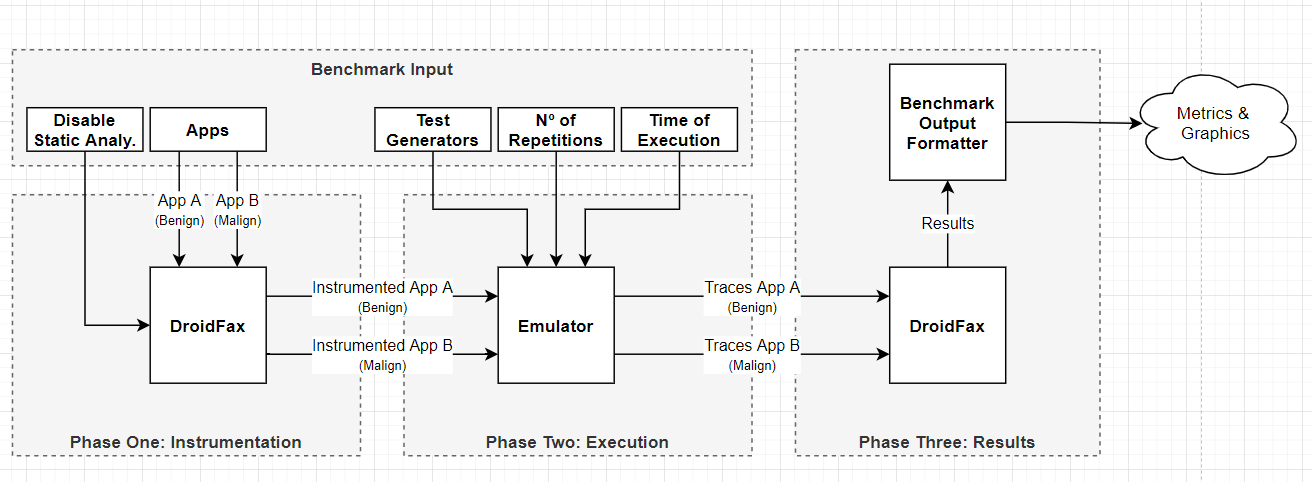
\includegraphics[width=1\textwidth]{images/benchmark4.png}
  \label{benchArq}
  \caption{DroidXP architecture}
  \label{fig:benchArq}
\end{figure*}

\subsubsection{Phase 1: Instrumentation}

In the first phase, a researcher must define the corpus of APK files DroidXP should consider during an
experiment execution. After that, DroidXP starts the DroidFax service that instruments each APK file,
so that DroidXP would be able to collect data (e.g., calls to sensitive APIs) about each execution.
To improve the performance of DroidXP, the instrumentation phase runs only once for each APK.
In this phase, the DroidFax tool also runs some static analysis procedures---when the
option \texttt{--disable-static-analysis} is not set.

\subsubsection{Phase 2: Execution}

In this phase, DroidXP installs an (already instrumented) APK file into
an Android emulator, and then executes a test case generation tool
during a period of time. This process repeats for every test case generation
tool and APK files. To provide repeatability of the experiment, DroidXP
removes all data stored in the emulator before starting
a new execution. That is, every execution uses a \emph{fresh} emulator,
without any information that might have been kept during
previous executions. 
It is relatively easy to add new test
case generation tools into DroidXP. Indeed,
every new tool must override two methods
of a \texttt{Tool} abstract class (according to
the Strategy Design pattern~\cite{patterns-book}.
%To carry out our replication study, we successfully integrated all
%test generation tools previously mentioned into DroidXP: Monkey, DroidBot, DroidMate, and
%Humanoid. 

\subsubsection{Phase 3: Result Analysis}

During the execution of the instrumented apps, all data that is relevant to our
research is collected by Logcat~\cite{Logcat}, one of the Android SDK's native tools. Logcat dumps a log from the Android emulator
while the already instrumented app is in execution. The part of the log we analyze in this phase comprises
the data sent by the methods within the Android app that were instrumented on the first
phase using the DroidFax tool. 

This data includes method coverage from the execution of each test generator tool and the
set of sensitive APIs the app calls during its execution. This set of calls to
sensitive APIs is necessary to estimate the test generator performance in identifying malicious apps---by spotting
differences between the sensitive API accessed by each version of an app (benign or malign).
In the end, DroidXP outputs the results of the experiment, which gives the
performance of one or more testing generator tools in mining sandboxes.

We used the DroidXP infrastructure to conduct our
first empirical study, whose settings we present in the following section. 

\subsection{First Study: A replication of the \blls}\label{sec:set1}

The \blls reports the results of an empirical study that compares the performance of test generation tools to mine Android
sandboxes~\cite{DBLP:conf/wcre/BaoLL18}. Since the \blls does not
compute the possible impact of DroidFax into the performance of the test generation tools,
here we replicate their work to understand the impact of the DroidFax static analysis algorithms into the \blls results.

Our replication differs from the original work in a few decisions. First, here we isolate
the effect of the DroidFax static analysis algorithms, in the task to identify malicious apps. In addition, although we use the same dataset of
$102$ pairs of Android apps used in the \blls, here we discarded $6$ pairs for which
we were not able to instrument---out of the $102$ pairs used in the original work, originally shared in the AndroZoo repository~\cite{DBLP:conf/msr/AllixBKT16}. We also introduced a recent test generator tool (Humanoid ~\cite{DBLP:conf/kbse/LiY0C19}), which
has not been considered in the previous work. Finally, we extended the execution time of each test generation tool,
executing each app from the test generation tool for three minutes (instead of one minute in the
original work),
and built the sandboxes after executing each test generation tool
three times---the original work executed each test generation tool
only once. It is important to note that our goal here is not to conduct an
exact replication of the \blls, but instead understand
the role of the DroidFax static analysis algorithms in the
performance of test case generation tools for mining sandboxes.
% The original study executed each app at each tool, for just one minute, and just one time.

Besides Humanoid, our study considers three test generation tools used in the \blls: DroidBot~\cite{DBLP:conf/icse/LiYGC17},
DroidMate~\cite{DBLP:conf/icse/JamrozikZ16}, and Monkey~\cite{Monkey}. We selected DroidBot and DroiMate because they achieved
the best performance on detecting malicious behavior---when considering the $102$ pairs of Android apps (B/M) in the \blls.
It is important to note that here we used a new version of DroidMate (DroidMate-2), since it presents several enhancements
in comparison to the previous version. We also considered the Google's Monkey open source tool, mostly because it is the most
widely used test generation tool for Android~\cite{DBLP:conf/sigsoft/ZengLZXDLYX16}. Monkey is part of the Android SDK
and does not require any additional installation effort. We included Humanoid in our study
because it is a recent tool that emulates realistic users, creating human-like test inputs using deep learning techniques.

\subsubsection{Data Collection}

Similarly to the \blls, besides
method coverage information, our experiments record every call
to \emph{sensitive methods} of the Android
platforms, while a given test case generation tool
is running. We consider the
same set of 97 sensitive methods 
from the AppGuard privacy-control framework
uses~\cite{DBLP:conf/esorics/BackesGHMS13}.

We executed DroidXP using two
configurations. In the first (named WOS), we executed DroidXP
using the dataset of 96 pairs of Android apps---each pair
including a benign and a malign version,
the four test case generation tools (DroidBot, DroidMate, Monkey, and Humanoid),
and the \texttt{--disable-static-analysis} option of
DroidFax, which disables the
execution of the DroidFax static analysis
component from the experiment. The WOS configuration
runs the test case generation tools for three times, using
a time limit of three minutes. 
In the second configuration (named WS), we executed DroidXP
using the same dataset of 96 pairs of Android apps, though 
executing only a fake test case generator tool (named Joker)
{\bf without} the \texttt{--disable-static-analysis} option.
Joker simulates a test tool that does not
run the Android apps during an experiment execution, and your use revealed the performance of static analysis component of DroidFax.

Using the WS configuration, the Execution Phase of
DroidXP does not collect any call to 
sensitive APIs, and thus we can estimate the performance of the
static analysis component of DroidFax (answering
RQ1).
Differently, the WOS configuration
disables the static analysis component of DroidFax and
we could better estimate the true performance of the test
case generation tools for mining android sandboxes 
(answering RQ2). For comparison purpose, we also
executed the four test case generation tools using the
DroidFax static analysis component. 


\subsubsection{Data Analysis} 

DroidXP produces a
dataset with the sensitive
APIs that the benign / malign
versions of an app call, during
the execution of each test case
generation tool. We estimate the
performance of a test case generation
tool by considering the percentage of
malwares in our dataset
its resulting sandbox is able to identify .

Recall that we build a sandbox 
during the exploratory phase of the mining
sandbox approach. This exploratory
phase records the set of 
sensitive APIs a benign version of an
app calls---during the execution of a test
case generation tool. Similarly to the \blls,
we consider that a sandbox of an
app identifies a malware whenever the
malicious version makes a call to a sensitive API  
that has not been recorded during the exploratory
phase (see Figure~\ref{fig:settings1}).

\begin{figure}
  \centering{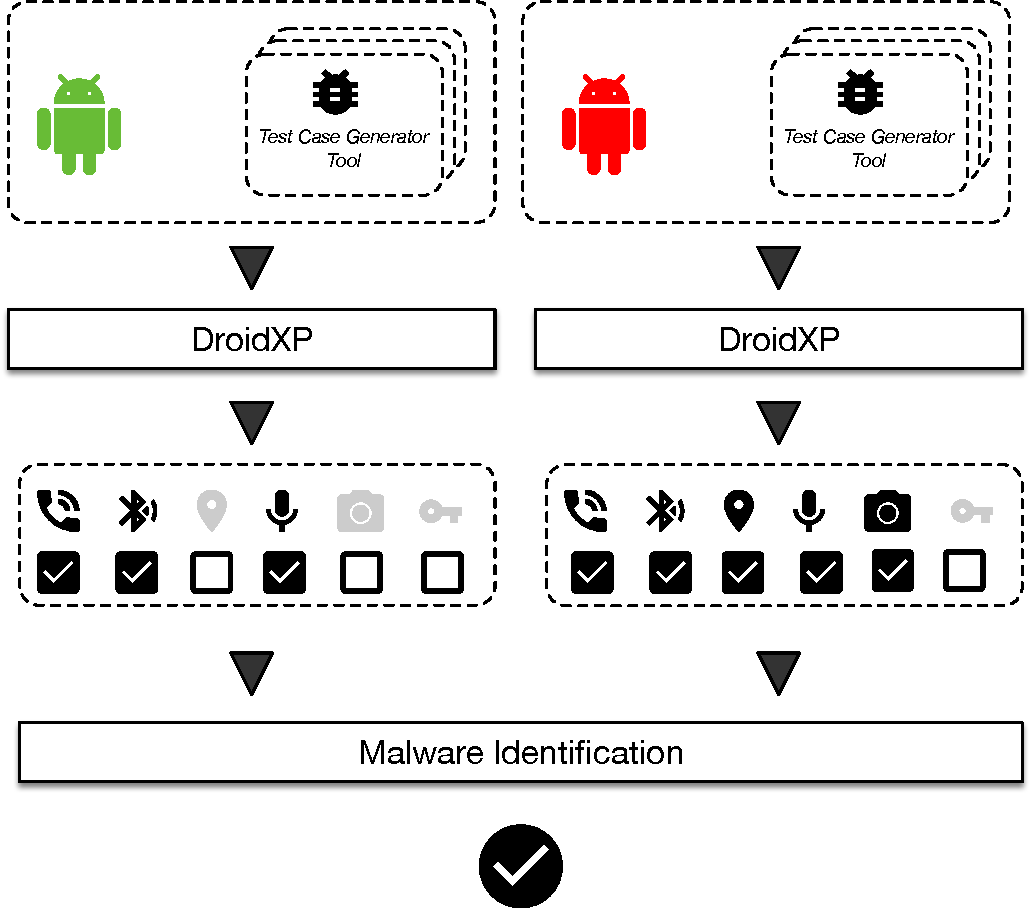
\includegraphics[scale=0.4]{images/first-study-settings.pdf}}
  \caption{Overview of our approach for malware identification in the first study.}
  \label{fig:settings1}
\end{figure}

To sum up, in order to analyse the
performance of the test case generation tools (including Joker),
we just have to compare the calls to sensitive APIs made by
the benign and malign versions of the apps, during
the execution of the tools. In the end, we generate
a set of observations, where each observation
contains the tool name, the number of the repetition (in the
range [1..3]), a boolean value reporting the use of the
DroidFax static analysis component, and a boolean value indicating
whether or not the malware has been identified. We use descriptive statistics
and plots to compare the performance of the tools and
answer RQ1 and RQ2. We also use \emph{Logistic Regression}~\cite[Chapter~4]{statistical-learning}
to understand the statistical relevance and
the contribution of each feature (tool, repetition, DroidFax static analysis
component) to malware identification. Our hypothesis here is that
the DroidFax static analysis component has a positive
effect on the performance of the sandboxes to identify malwares. 

\subsection{Second Study: Use of Taint Analysis for Malware Identification}\label{sec:set2}

In the second empirical study 
we investigate whether or not a taint-based static analysis approach is also promising for
identifying malwares, given a version of an app that we can assume to be secure (goal of research
question RQ3).
To this end, we leverage the FlowDroid
taint analysis algorithms for Android apps (version 2.8), in order to identify dataflows
that might lead to the leakage of sensitive information. Our
goal here is to investigate if it is possible to detect malicious
behavior by means of the \emph{divergent} source-sink paths that FlowDroid reveals after
analysing a benign and a malign versions of an Android app.

\subsubsection{Data Collection}

FlowDroid takes as input an Android Application Package (APK file) and
a set of API methods marked either as {\bf source}
or {\bf sink} (or both). Source methods are those that access \emph{sensitive information} (e.g.,
a method that access the user location), while sink methods are those 
that \emph{might share information with external peers} (e.g., a method that
sends messages to a recipient). We rely on the source-sink definitions
of the FlowDroid implementation~\cite{arzt:pldi-2014,rasthofer-source-sink},
which involves a curate list of source and sink methods (including callbacks and
other Android API methods of interest).
FlowDroid then uses a \emph{context, flow, and field
sensitive analysis} to identify dataflow paths from sources to sinks~\cite{arzt:pldi-2014}.

Our data collection approach involves three steps (see Figure~\ref{fig:settings2}). In the first, we execute FlowDroid to mine the source-sink paths from a benign version of an app, and then enumerate a set (S1) with the 
possible dataflows between sources and sinks. All paths in S1 are considered secure
in our analysis. In the second step we repeat the FlowDroid execution, though
considering the malicious APK version of the app.
This leads to a second set (S2) of source-sink paths.

It is important to note that not all source-sink paths are malign, and then we
follow a specific methodology to identify malwares using taint analysis. That is,
we only report a malware when
FlowDroid finds an additional source-sink path in the malicious version of an app, which
has not been identified when analysing the benign version. Therefore, in the third step we compute the difference (S3) between the sets S2 and S1 (i.e., $S3 = S2 \setminus S1$). If the set S3 is not empty, we assume that FlowDroid
has identified the malware.

In this second study we use the same dataset of $96$ pairs of Android apps (B/M) used in the first empirical
study.


\begin{figure}
  \centering{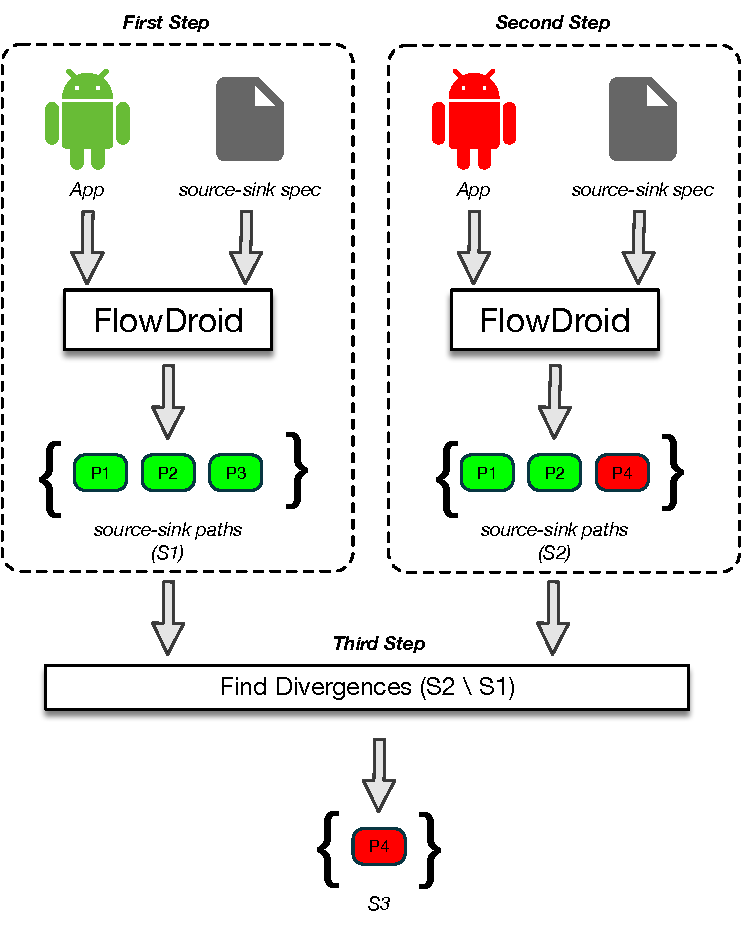
\includegraphics[scale=0.4]{images/second-study-settings.pdf}}
  \caption{Overview of our approach in the second study.}
  \label{fig:settings2}
\end{figure}


\subsubsection{Data analysis}


We use two metrics in this second study:
the total number of malicious apps FlowDroid is able to
find and the execution time for running the taint analysis algorithm
for each app. Similarly to the first empirical study,
we use descriptive statistics
and plots to compare the performance of the taint analysis and
mining sandbox approaches. We also use \emph{Logistic Regression}~\cite[Chapter~4]{statistical-learning}
to better understand the statistical
significance of the benefits of using FlowDroid
(in comparison to the DroidFax static analysis
component only). Our hypothesis here is that
FlowDroid outperforms, in terms of the number of
detected malware, the sandbox generated
by the DroidFax static analysis component. 
